\chapter{जैव-अणु: ऐमीनो अम्ल, शर्कराएँ, लिपिड और न्यूक्लियोटाइड}\label{ch:b2:biomolecules}

एक सामान्य मधुरक, जो शक्कर से कहीं अधिक मीठा है, एक अकेले ऐमाइड आबंध से जुड़े दो ऐमीनो अम्ल हैं, जिनमें से एक
अपने मेथिल एस्टर के रूप में है: ऐस्पार्टिक अम्ल और फ़ेनिलऐलानीन, दोनों उस विन्यास के साथ जिसे सजीव कोशिकाएँ
प्रयुक्त करती हैं। जीवन के अणु छोटी इकाइयों के कुछ परिवारों से बने हैं, ऐमीनो अम्ल, शर्कराएँ, \omterm{def:b2:biomolecules:lipid}{वसा
अम्ल} और \omterm{def:b2:biomolecules:nucleotide}{न्यूक्लियोटाइड}, जो पिछले अध्यायों की अभिक्रियाओं से जुड़े हैं: ऐमाइड, ऐसीटैल, एस्टर। यह
अध्याय उन्हें वैसे पढ़ता है जैसे कोई कार्बनिक रसायनज्ञ पढ़ता है: क्रियात्मक समूह, त्रिविम-रसायन, अम्ल--क्षारक
व्यवहार, और वे अभिक्रियाएँ जो उन्हें जोड़ती और काटती हैं।
% ledger: use:aspartame

\begin{recall}
प्रथम वर्ष का खंड: CIP नियम, फ़िशर प्रक्षेप, किरैलता, हेमीऐसीटैल और ऐसीटैल, $\mathrm pK_a$
और वितरण आरेख, उभयरागी अणु, बायो का नियम। \Cref{ch:b2:acyl-substitution}: ऐमाइड,
एस्टर, \omterm{def:b2:acyl-substitution:saponification}{साबुनीकरण}, सक्रियित अम्ल। \Cref{ch:b2:amines}: क्षारक के रूप में ऐमीन।
\Cref{ch:b2:retrosynthesis}: किसी मार्ग में रक्षी समूह।
\end{recall}

\section{ऐमीनो अम्ल}

\begin{definition}[ऐमीनो अम्ल]\label{def:b2:biomolecules:amino-acid}
\emph{$\alpha$-ऐमीनो अम्ल}\index{अल्फ़ा-ऐमीनो अम्ल@$\alpha$-ऐमीनो अम्ल} \ce{H2N-CHR-COOH} एक ही कार्बन पर एक
ऐमीनो समूह और एक कार्बोक्सिलिक अम्ल समूह धारण करता है; \ce{R} उसकी \emph{पार्श्व
शृंखला}\index{पार्श्व शृंखला} है। उदासीन pH के निकट जल में यह \emph{उभयाविष्ट आयन}\index{उभयाविष्ट आयन} के रूप में रहता है,
\ce{H3N+-CHR-COO-}, जो एक धनात्मक और एक ऋणात्मक आवेश धारण करता है। \emph{समविभव
बिंदु}\index{समविभव बिंदु} pI वह pH है जिस पर इसका औसत शुद्ध आवेश शून्य है।
\end{definition}

सजीवों के प्रोटीन बीस ऐमीनो अम्लों से बनते हैं। ग्लाइसीन (\ce{R = H}) को छोड़कर सभी किरैल हैं, और
प्राकृतिक ऐमीनो अम्लों का विन्यास L है (\cref{def:b2:biomolecules:d-l})। उनकी पार्श्व शृंखलाएँ उन्हें
परिवारों में बाँटती हैं: अध्रुवी (ऐलानीन, \ce{R = CH3}; फ़ेनिलऐलानीन, \ce{R = CH2C6H5}), ध्रुवी, अम्लीय
(ऐस्पार्टिक और ग्लूटैमिक अम्ल, एक दूसरे कार्बोक्सिलिक समूह के साथ) और क्षारकीय (लाइसीन, एक दूसरे ऐमीनो
समूह के साथ; हिस्टिडीन, एक इमिडैज़ोल वलय के साथ)।

\begin{proposition}[समविभव बिंदु]\label{prop:b2:biomolecules:pi}
ऐसी \omterm{def:b2:biomolecules:amino-acid}{पार्श्व शृंखला} वाले ऐमीनो अम्ल के लिए जो न अम्लीय है न क्षारकीय, $\mathrm{pI} = (\mathrm pK_{a1} +
\mathrm pK_{a2})/2$, जहाँ $\mathrm pK_{a1}$ कार्बोक्सिलिक समूह का है और $\mathrm pK_{a2}$
अमोनियम समूह का। अम्लीय या क्षारकीय \omterm{def:b2:biomolecules:amino-acid}{पार्श्व शृंखला} के लिए pI उन दो $\mathrm pK_a$ का माध्य है जो
उदासीन रूप को घेरते हैं।
\end{proposition}

\begin{proof}
धनायन के लिए \ce{H2A+}, \omterm{def:b2:biomolecules:amino-acid}{उभयाविष्ट आयन} के लिए \ce{HA} और ऋणायन के लिए \ce{A-} लिखिए। शुद्ध आवेश
शून्य होता है जब $[\ce{H2A+}] = [\ce{A-}]$। $K_{a1} = [\ce{HA}]h/[\ce{H2A+}]$ और $K_{a2} =
[\ce{A-}]h/[\ce{HA}]$ से, $h = [\ce{H3O+}]$ के साथ, अनुपात $[\ce{H2A+}]/[\ce{A-}] = h^2/(K_{a1}K_{a2})$
$h^2 = K_{a1}K_{a2}$ के लिए 1 के बराबर है, अर्थात् $\mathrm{pH} = (\mathrm pK_{a1} + \mathrm pK_{a2})/2$। किसी
तीसरे आयननीय समूह के साथ यही तर्क उदासीन रूप के दोनों ओर के दो साम्यों पर लागू होता है,
तब तीसरा समूह पूर्णतः एक ही अवस्था में होता है।
\end{proof}

ग्लाइसीन के लिए $\mathrm pK_{a1} = 2.35$ और $\mathrm pK_{a2} = 9.78$: pI $\approx 6.1$। ऐस्पार्टिक अम्ल
(2.0, 3.9, 9.9) का pI $\approx 3.0$ है; लाइसीन (2.2, 9.1, 10.7) का pI $\approx 9.9$ है।
% ledger: pka:glycine1, pka:glycine2, pka:asp1, pka:asp2, pka:asp3, pka:lys1, pka:lys2, pka:lys3

\begin{omfigure}
\begin{tikzpicture}
\begin{axis}[width=0.47\linewidth, height=5cm, xmin=0, xmax=14, ymin=-2.2, ymax=2.2,
  xlabel={pH}, ylabel={शुद्ध आवेश}, label style={font=\small}, tick label style={font=\scriptsize},
  xtick={0,2,4,6,8,10,12,14}, ytick={-2,-1,0,1,2}, grid=major, grid style={black!12},
  legend style={font=\scriptsize, at={(0.5,1.03)}, anchor=south}, legend columns=3]
\addplot[omDef, thick] table[x=pH, y=gly] {figdata/out/bachelor-2-amino-acid-charge-a.dat};
\addplot[omThm, thick] table[x=pH, y=asp] {figdata/out/bachelor-2-amino-acid-charge-a.dat};
\addplot[omMeth, thick] table[x=pH, y=lys] {figdata/out/bachelor-2-amino-acid-charge-a.dat};
\legend{ग्लाइसीन, ऐस्पार्टिक अम्ल, लाइसीन}
\end{axis}
\end{tikzpicture}\hfill
\begin{tikzpicture}
\begin{axis}[width=0.47\linewidth, height=5cm, xmin=0, xmax=14, ymin=0, ymax=1.05,
  xlabel={pH}, ylabel={अंश}, label style={font=\small}, tick label style={font=\scriptsize},
  xtick={0,2,4,6,8,10,12,14},
  legend style={font=\scriptsize, at={(0.5,1.03)}, anchor=south}, legend columns=3]
\addplot[omThm, thick] table[x=pH, y=cation] {figdata/out/bachelor-2-amino-acid-charge-b.dat};
\addplot[omDef, thick] table[x=pH, y=zwitterion] {figdata/out/bachelor-2-amino-acid-charge-b.dat};
\addplot[omMeth, thick] table[x=pH, y=anion] {figdata/out/bachelor-2-amino-acid-charge-b.dat};
\legend{धनायन, उभयाविष्ट आयन, ऋणायन}
\end{axis}
\end{tikzpicture}

{\small बाएँ: \qty{25}{\degreeCelsius} पर उनके $\mathrm pK_a$ से, pH के विरुद्ध तीन ऐमीनो अम्लों का
शुद्ध आवेश; हर वक्र pI पर शून्य को काटता है। दाएँ: ग्लाइसीन के तीन रूप,
\ce{H3N+CH2COOH}, \ce{H3N+CH2COO-} और \ce{H2NCH2COO-}; \omterm{def:b2:biomolecules:amino-acid}{उभयाविष्ट आयन} लगभग pH 3 से
pH 9 तक प्रभावी है।}
% figdata: bachelor-2/amino-acid-charge.py parts a, b
\end{omfigure}

\begin{method}[किसी दिए गए pH पर शुद्ध आवेश]\label{met:b2:biomolecules:charge}
\begin{enumerate}
  \item हर आयननीय समूह को उसके $\mathrm pK_a$ के साथ सूचीबद्ध कीजिए: अंतस्थ \ce{NH3+} और \ce{COOH}, और
        आयननीय पार्श्व शृंखलाएँ।
  \item हर समूह के लिए pH और $\mathrm pK_a$ की तुलना कीजिए: कोई समूह अपने
        $\mathrm pK_a$ से नीचे अधिकांशतः प्रोटॉनित होता है, ऊपर अधिकांशतः विप्रोटॉनित (1 इकाई से अधिक के अंतर पर: 90~\% से अधिक)।
  \item आवेश जोड़िए: \ce{NH3+} $+1$, \ce{NH2} 0, \ce{COOH} 0, \ce{COO-} $-1$ (इमिडैज़ोलियम $+1$)।
  \item किसी $\mathrm pK_a$ के निकट उस समूह को आधा आवेशित गिनिए; यथातथ मान के लिए अंश
        $1/(1 + 10^{\mathrm pK_a - \mathrm{pH}})$ प्रयुक्त कीजिए।
\end{enumerate}
\end{method}

\section{पेप्टाइड}

\begin{definition}[पेप्टाइड]\label{def:b2:biomolecules:peptide}
एक ऐमीनो अम्ल के कार्बोक्सिलिक समूह और दूसरे के ऐमीनो समूह के बीच बना ऐमाइड आबंध
\emph{पेप्टाइड आबंध}\index{पेप्टाइड आबंध} है; पेप्टाइड आबंधों से जुड़े ऐमीनो अम्लों की शृंखला
\emph{पेप्टाइड}\index{पेप्टाइड} है (लंबी होने पर प्रोटीन), जो अपने मुक्त ऐमीनो सिरे (N-अंत्य)
से अपने मुक्त कार्बोक्सिलिक सिरे (C-अंत्य) तक लिखी जाती है। \emph{पेप्टाइड युग्मन}\index{पेप्टाइड युग्मन}
प्रयोगशाला में किसी \emph{युग्मन अभिकर्मक}\index{युग्मन अभिकर्मक} से पेप्टाइड आबंध बनाता है, जो ऐसा अभिकर्मक है
जो मृदु परिस्थितियों में कार्बोक्सिलिक समूह को सक्रियित व्युत्पन्न में बदल देता है (उदाहरण के लिए कोई
कार्बोडाइइमाइड)।
\end{definition}

\begin{omfigure}
\setchemfig{atom sep=1.9em}
\schemestart
\chemfig{R-C(=[2]O)-N(-[6]H)-R'}
\arrow{<->}
\chemfig{R-C(-[2]\chemabove{O}{\scriptstyle -})=\chemabove{N}{\scriptstyle +}(-[6]H)-R'}
\schemestop
\par\vspace{6pt}

{\small \omterm{def:b2:biomolecules:peptide}{पेप्टाइड आबंध} की दो अनुनादी संरचनाएँ। नाइट्रोजन का एकाकी युग्म
कार्बोनिल के साथ साझा होता है: \ce{C-N} आबंध में आंशिक द्वि-आबंध लक्षण है, और छह परमाणु C, C, O, N, H, C
एक तल में होते हैं।}
\end{omfigure}

\begin{proposition}[एक समतलीय आबंध]\label{prop:b2:biomolecules:planar}
\omterm{def:b2:biomolecules:peptide}{पेप्टाइड आबंध} समतलीय है, \ce{C-N} आबंध के परितः घूर्णन प्रतिबंधित है, और ऐमाइड नाइट्रोजन
न क्षारकीय है न नाभिकरागी।
\end{proposition}

\begin{proof}[तर्क]
दूसरी अनुनादी संरचना \ce{C-N} आबंध को द्वि-आबंध लक्षण का एक भाग देती है: इसे घुमाने से
नाइट्रोजन के एकाकी युग्म का \ce{C=O} $\pi$ निकाय के साथ अतिव्यापन टूट जाता, जिसमें ऊर्जा लगती है, अतः
उसके आसपास के परमाणु एक तल में रहते हैं, और trans व्यवस्था (दोनों शृंखला कार्बन
\ce{C-N} आबंध की विपरीत ओर) सामान्य है। अनुनाद में लगा एकाकी युग्म किसी प्रोटॉन या
इलेक्ट्रॉनरागी के लिए उपलब्ध नहीं है, जैसा हर ऐमाइड के लिए है (\cref{ch:b2:acyl-substitution})। प्रोटीन इन
दृढ़ तलों की शृंखलाओं के चारों ओर मुड़ते हैं।
\end{proof}

\begin{proposition}[रक्षण और सक्रियण क्यों]\label{prop:b2:biomolecules:coupling}
दो ऐमीनो अम्लों से कोई एक निर्धारित डाइपेप्टाइड बनाने के लिए उन समूहों का रक्षण आवश्यक है जिन्हें
अभिक्रिया नहीं करनी चाहिए और उस कार्बोक्सिलिक समूह का सक्रियण भी जिसे करनी चाहिए।
\end{proposition}

\begin{proof}[तर्क]
कमरे के ताप पर मिलाए गए कार्बोक्सिलिक अम्ल और ऐमीन लवण देते हैं, ऐमाइड नहीं; जल को निकालने के लिए गर्म करने से
ऐमीनो अम्ल रेसेमिक भी हो जाते। अतः सक्रियण (\omterm{def:b2:acyl-substitution:derivative}{ऐसिल क्लोराइड}, ऐनहाइड्राइड, या \omterm{def:b2:biomolecules:peptide}{युग्मन
अभिकर्मक}) आवश्यक है। परंतु हर ऐमीनो अम्ल में दोनों समूह हैं: ग्लाइसीन और
ऐलानीन के मिश्रण को सक्रिय करने से Gly--Ala, Ala--Gly, Gly--Gly, Ala--Ala और लंबी शृंखलाएँ मिलतीं। पहले के
ऐमीन और दूसरे के अम्ल को अवरुद्ध करने से केवल एक संभव आबंध बचता है।
\end{proof}

\begin{method}[डाइपेप्टाइड का संश्लेषण]\label{met:b2:biomolecules:peptide}
\begin{enumerate}
  \item N-अंत्य ऐमीनो अम्ल के ऐमीनो समूह का रक्षण कीजिए (कार्बामेट के रूप में, उदाहरण के लिए एक
        \textit{tert}-ब्यूटॉक्सीकार्बोनिल समूह)।
  \item C-अंत्य ऐमीनो अम्ल के कार्बोक्सिलिक समूह का रक्षण कीजिए (मेथिल या बेन्ज़िल एस्टर के रूप में), और किसी भी
        अभिक्रियाशील \omterm{def:b2:biomolecules:amino-acid}{पार्श्व शृंखला} का।
  \item मुक्त कार्बोक्सिलिक समूह को \omterm{def:b2:biomolecules:peptide}{युग्मन अभिकर्मक} से सक्रिय कीजिए और रक्षित भागीदार मिलाइए: एक
        \omterm{def:b2:biomolecules:peptide}{पेप्टाइड आबंध} बनता है।
  \item रक्षी समूह हटाइए, अधिमानतः एक लांबिक समुच्चय
        (\cref{def:b2:retrosynthesis:orthogonal}); आगे बढ़ने के लिए केवल ऐमीन का रक्षण हटाइए और दोहराइए।
\end{enumerate}
\end{method}

विलयन में चक्र को कई बार दोहराने के लिए हर चरण पर शोधन की आवश्यकता होती। ठोस-प्रावस्था
संश्लेषण में बढ़ती शृंखला अपने C-अंत्य द्वारा किसी \omterm{def:b2:polymer-synthesis:polymer}{बहुलक} मनके से जुड़ी होती है; आधिक्य अभिकर्मक और
उपोत्पाद हर युग्मन के बाद धो दिए जाते हैं, और तैयार \omterm{def:b2:biomolecules:peptide}{पेप्टाइड} को अंत में आधार से
काट लिया जाता है।

\begin{omfigure}
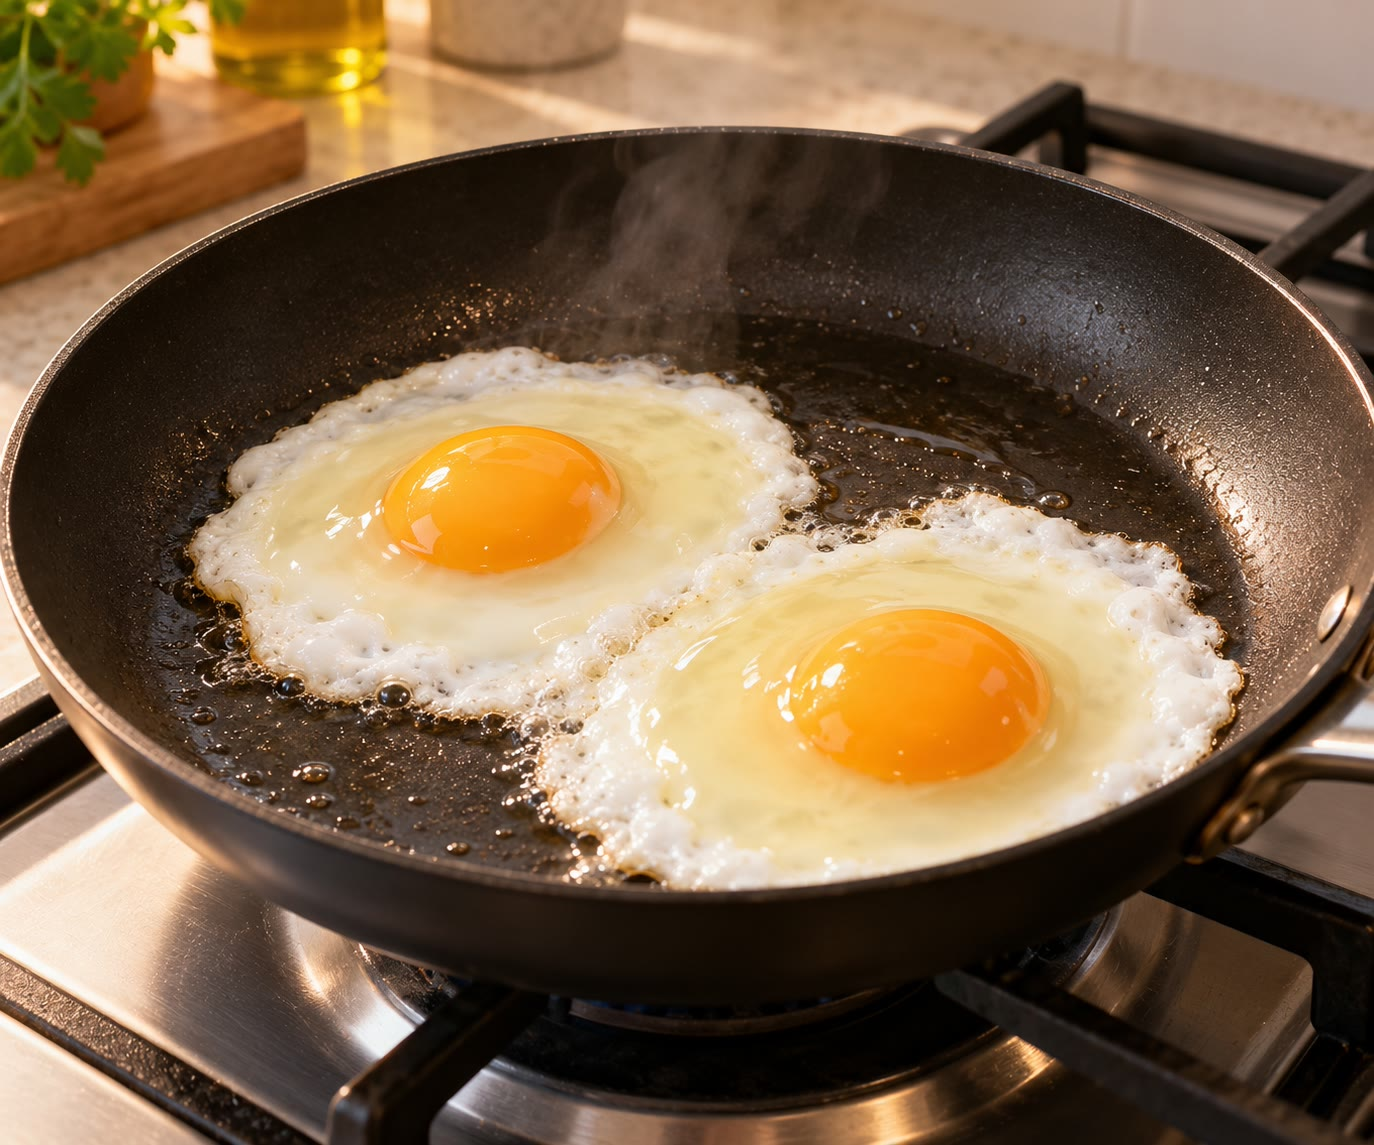
\includegraphics[width=0.5\linewidth]{images/book3/ai/b2-30-eggs.jpg}

{\small तलते हुए अंडे। सफ़ेदी के प्रोटीन गर्म करने पर खुल जाते हैं और एक-दूसरे से जुड़ जाते हैं:
पारभासी द्रव एक अपारदर्शी सफ़ेद ठोस में बदल जाता है। कोई \omterm{def:b2:biomolecules:peptide}{पेप्टाइड आबंध} नहीं टूटता; परिवर्तन इस बात में है कि
शृंखलाएँ कैसे मुड़ी हुई हैं (चित्रण)।}
\end{omfigure}

\section{कार्बोहाइड्रेट}

\begin{definition}[D और L]\label{def:b2:biomolecules:d-l}
किसी शर्करा या ऐमीनो अम्ल को फ़िशर प्रक्षेप में उसके सबसे अधिक ऑक्सीकृत कार्बन को शीर्ष पर रखकर खींचा जाता है। वह
D है यदि शीर्ष से सबसे दूर वाले त्रिविमजनक केंद्र पर \ce{OH} (या, किसी $\alpha$-ऐमीनो अम्ल के लिए,
$\alpha$ कार्बन पर \ce{NH2}) दाईं ओर इंगित करता है, और L यदि बाईं ओर। ये वर्णनक
विन्यासों की तुलना ग्लिसरैल्डिहाइड के विन्यास से करते हैं; ये CIP वर्णनक नहीं हैं।
\end{definition}

\begin{definition}[मोनोसैकेराइड]\label{def:b2:biomolecules:sugar}
\emph{मोनोसैकेराइड}\index{मोनोसैकेराइड} एक पॉलिहाइड्रॉक्सी ऐल्डिहाइड या कीटोन है, प्रायः
\ce{C_nH_{2n}O_n}, $n$ 3 से 7 तक, जिसका छोटी शर्कराओं में जल-अपघटन नहीं हो सकता।
\emph{ऐल्डोस}\index{ऐल्डोस} के C1 पर ऐल्डिहाइड समूह होता है, \emph{कीटोस}\index{कीटोस} के कीटोन समूह,
प्रायः C2 पर। ग्लूकोस एक ऐल्डोहेक्सोस है, फ़्रक्टोस एक कीटोहेक्सोस।
\end{definition}

जल में कोई ऐल्डोहेक्सोस लगभग पूर्णतः चक्रीय होता है: C5 पर का \ce{OH} ऐल्डिहाइड से जुड़कर
एक षट्सदस्यी हेमीऐसीटैल वलय (एक पाइरैनोस) बनाता है। चक्रीकरण C1 पर एक नया त्रिविमजनक केंद्र बनाता है।

\begin{definition}[ऐनोमर]\label{def:b2:biomolecules:anomer}
\emph{हॉवर्थ प्रक्षेप}\index{हॉवर्थ प्रक्षेप} में किसी चक्रीय शर्करा का वलय सपाट खींचा जाता है,
पृष्ठ के लंबवत, उसका ऑक्सीजन पीछे दाईं ओर और उसके प्रतिस्थापी वलय के ऊपर या नीचे।
हेमीऐसीटैल कार्बन (किसी \omterm{def:b2:biomolecules:sugar}{ऐल्डोस} का C1) \emph{ऐनोमरी कार्बन}\index{ऐनोमरी कार्बन} है; इसके
दो संभव विन्यास दो अप्रतिबिंबी त्रिविम समावयवी देते हैं, अर्थात् \emph{ऐनोमर}\index{ऐनोमर}: किसी D
शर्करा के लिए $\alpha$ में ऐनोमरी \ce{OH} वलय के नीचे होता है (\ce{CH2OH} के विपरीत), $\beta$ में ऊपर।
जल में ऐनोमर खुली शृंखला से होकर परस्पर बदलते हैं, और ताज़ा घोले गए
ऐनोमर का ध्रुवण घूर्णन धीरे-धीरे एक साम्य मान तक खिसकता है: \emph{परिवर्ती घूर्णन}\index{परिवर्ती घूर्णन}।
\end{definition}

\begin{omfigure}
\setchemfig{atom sep=1.7em}
\begin{minipage}[c]{0.24\linewidth}\centering
\chemfig{CHO-[6]C(-[4]H)(-[0]OH)-[6]C(-[4,,,2]HO)(-[0]H)-[6]C(-[4]H)(-[0]OH)-[6]C(-[4]H)(-[0]OH)-[6]CH_2OH}
\end{minipage}%
\begin{minipage}[c]{0.37\linewidth}\centering
\begin{tikzpicture}[x=1cm, y=1cm, font=\small]
\coordinate (C4) at (-1.5,0); \coordinate (C3) at (-0.75,-0.65); \coordinate (C2) at (0.75,-0.65);
\coordinate (C1) at (1.5,0); \coordinate (O) at (0.75,0.45); \coordinate (C5) at (-0.75,0.45);
\draw (C5) -- (O) -- (C1); \draw (C4) -- (C5);
\draw[line width=2.2pt] (C4) -- (C3) -- (C2) -- (C1);
\node[fill=white, inner sep=1pt] at (O) {O};
\draw (C5) -- ++(0,0.6) node[above] {\ce{CH2OH}};
\draw (C1) -- ++(0,-0.6) node[below] {OH}; \draw (C1) -- ++(0,0.5) node[above] {H};
\draw (C2) -- ++(0,-0.6) node[below] {OH}; \draw (C3) -- ++(0,0.35) node[above, inner sep=1pt] {OH};
\draw (C4) -- ++(0,-0.6) node[below] {OH};
\node at (0,-2.0) {$\alpha$-D-ग्लूकोपाइरैनोस};
\end{tikzpicture}
\end{minipage}%
\begin{minipage}[c]{0.37\linewidth}\centering
\begin{tikzpicture}[x=1cm, y=1cm, font=\small]
\coordinate (C4) at (-1.5,0); \coordinate (C3) at (-0.75,-0.65); \coordinate (C2) at (0.75,-0.65);
\coordinate (C1) at (1.5,0); \coordinate (O) at (0.75,0.45); \coordinate (C5) at (-0.75,0.45);
\draw (C5) -- (O) -- (C1); \draw (C4) -- (C5);
\draw[line width=2.2pt] (C4) -- (C3) -- (C2) -- (C1);
\node[fill=white, inner sep=1pt] at (O) {O};
\draw (C5) -- ++(0,0.6) node[above] {\ce{CH2OH}};
\draw (C1) -- ++(0,0.5) node[above] {OH}; \draw (C1) -- ++(0,-0.6) node[below] {H};
\draw (C2) -- ++(0,-0.6) node[below] {OH}; \draw (C3) -- ++(0,0.35) node[above, inner sep=1pt] {OH};
\draw (C4) -- ++(0,-0.6) node[below] {OH};
\node at (0,-2.0) {$\beta$-D-ग्लूकोपाइरैनोस};
\end{tikzpicture}
\end{minipage}
\par\vspace{6pt}

{\small D-ग्लूकोस। बाएँ: फ़िशर प्रक्षेप में खुली शृंखला, C5 पर \ce{OH} दाईं ओर (D)। मध्य
और दाएँ: \omterm{def:b2:biomolecules:anomer}{हॉवर्थ प्रक्षेप} में दोनों पाइरैनोस \omterm{def:b2:biomolecules:anomer}{ऐनोमर}; फ़िशर
प्रक्षेप में दाईं ओर वाले समूह नीचे इंगित करते हैं, बाईं ओर वाले ऊपर, और C5 \ce{CH2OH} को ऊपर रखता है। \omterm{def:b2:biomolecules:anomer}{ऐनोमर}
केवल C1 पर भिन्न हैं। C2 से C5 तक के हाइड्रोजन छोड़ दिए गए हैं।}
\end{omfigure}

\begin{method}[फ़िशर से हॉवर्थ तक (D-ऐल्डोपाइरैनोस)]\label{met:b2:biomolecules:haworth}
\begin{enumerate}
  \item वलय को ऐसे खींचिए कि O पीछे दाईं ओर हो, C1 दाईं ओर, फिर C2, C3, C4 दक्षिणावर्त सामने
        और बाईं ओर, C5 पीछे बाईं ओर।
  \item फ़िशर प्रक्षेप में दाईं ओर वाले समूह नीचे जाते हैं, बाईं ओर वाले ऊपर।
  \item C5 पर (D श्रेणी) \ce{CH2OH} ऊपर जाता है।
  \item C1 पर \ce{OH} $\alpha$ के लिए नीचे जाता है, $\beta$ के लिए ऊपर।
\end{enumerate}
\end{method}

\begin{proposition}[परिवर्ती घूर्णन साम्य]\label{prop:b2:biomolecules:mutarotation}
यदि शुद्ध \omterm{def:b2:biomolecules:anomer}{ऐनोमरों} के विशिष्ट घूर्णन $[\alpha]_\alpha$ और $[\alpha]_\beta$ हों और
साम्य मिश्रण का $[\alpha]_{\mathrm{eq}}$, तो साम्य पर $\alpha$ \omterm{def:b2:biomolecules:anomer}{ऐनोमर} का मोल अंश
यह है:
\begin{equation*}
x_\alpha = \frac{[\alpha]_{\mathrm{eq}} - [\alpha]_\beta}{[\alpha]_\alpha - [\alpha]_\beta}.
\end{equation*}
\end{proposition}

\begin{proof}
खुली शृंखला मिश्रण का अत्यल्प अंश है और उसकी उपेक्षा की जाती है। दोनों \omterm{def:b2:biomolecules:anomer}{ऐनोमरों} के घूर्णन
उनकी सांद्रताओं के अनुपात में जुड़ते हैं (बायो का नियम, प्रथम वर्ष का खंड); चूँकि उनका मोलर
द्रव्यमान समान है, $[\alpha]_{\mathrm{eq}} = x_\alpha[\alpha]_\alpha + (1 - x_\alpha)[\alpha]_\beta$, जिसे
$x_\alpha$ के लिए हल किया जाता है।
\end{proof}

जल में साम्य पर D-ग्लूकोस का $[\alpha] = +52.7$ है (\unit{\degree\,dm^{-1}\,g^{-1}\,mL} में)।
$+112$ और $+18.7$ (अभ्यास के आँकड़े) के \omterm{def:b2:biomolecules:anomer}{ऐनोमर} घूर्णनों के साथ $x_\alpha = (52.7 - 18.7)/(112 - 18.7)
\approx 0.36$: लगभग 36~\% $\alpha$ और 64~\% $\beta$। $\beta$ \omterm{def:b2:biomolecules:anomer}{ऐनोमर}, जिसके सभी
प्रतिस्थापी कुर्सी रूप में विषुवतीय हैं, अधिक स्थायी है।
% ledger: rot:glucose-eq

\begin{definition}[ग्लाइकोसाइड]\label{def:b2:biomolecules:glycoside}
\emph{ग्लाइकोसाइड}\index{ग्लाइकोसाइड} वह ऐसीटैल है जो तब बनता है जब किसी शर्करा का ऐनोमरी \ce{OH}
किसी ऐल्कोहॉल, प्रायः किसी अन्य शर्करा, के \ce{OR} समूह से प्रतिस्थापित होता है; \omterm{def:b2:biomolecules:anomer}{ऐनोमरी कार्बन} से उस
ऑक्सीजन तक का आबंध \emph{ग्लाइकोसाइडी आबंध}\index{ग्लाइकोसाइडी आबंध} है। \emph{अपचायी शर्करा}\index{अपचायी शर्करा}
वह है जो फ़ेलिंग विलयन या टॉलेन्स अभिकर्मक जैसे मृदु ऑक्सीकारकों का अपचयन करती है।
\end{definition}

\begin{proposition}[अपचायी या नहीं]\label{prop:b2:biomolecules:reducing}
मुक्त हेमीऐसीटैल (या हेमीकीटैल) समूह वाली शर्करा अपचायी है; वह \omterm{def:b2:biomolecules:glycoside}{ग्लाइकोसाइड} जिसके सभी \omterm{def:b2:biomolecules:anomer}{ऐनोमरी कार्बन}
\omterm{def:b2:biomolecules:glycoside}{ग्लाइकोसाइडी आबंधों} में लगे हों, अपचायी नहीं है।
\end{proposition}

\begin{proof}[तर्क]
हेमीऐसीटैल खुली शृंखला के साथ साम्य में होता है, जिसके ऐल्डिहाइड समूह को अभिकर्मक ऑक्सीकृत करता है;
फिर साम्य और वलयों को खोलता है जब तक सारी शर्करा अभिक्रिया न कर ले। ऐसीटैल
उदासीन या क्षारीय जल में नहीं खुलता: \omterm{def:b2:biomolecules:anomer}{ऐनोमरी कार्बन} बंद रहता है, और ऑक्सीकृत करने के लिए कोई ऐल्डिहाइड नहीं होता।
\end{proof}

माल्टोस (दो ग्लूकोस, एक का C1 दूसरे के O4 से आबंधित) एक मुक्त हेमीऐसीटैल बनाए रखता है और अपचायी है;
सुक्रोस ग्लूकोस और फ़्रक्टोस के \omterm{def:b2:biomolecules:anomer}{ऐनोमरी कार्बनों} को आपस में जोड़ता है और अपचायी नहीं है। स्टार्च और
सेलुलोस दोनों C1--O4 जुड़े ग्लूकोस की शृंखलाएँ हैं: स्टार्च में $\alpha$, जो कुंडलित होता है और पचता है;
सेलुलोस में $\beta$, जिसकी सीधी शृंखलाएँ हाइड्रोजन आबंधों से थमे रेशों में संकुलित होती हैं।

\section{लिपिड}

\begin{definition}[लिपिड]\label{def:b2:biomolecules:lipid}
\emph{वसा अम्ल}\index{वसा अम्ल} लंबी अशाखित शृंखला वाला कार्बोक्सिलिक अम्ल है, प्रायः 12 से
22 कार्बनों की, संतृप्त या (\textit{Z}) द्वि-आबंधों वाली। \emph{ट्राइग्लिसराइड}\index{ट्राइग्लिसराइड}
प्रोपेन-1,2,3-ट्राइऑल (ग्लिसरॉल) का तीन वसा अम्लों के साथ ट्राइएस्टर है।
\emph{फ़ॉस्फ़ोलिपिड}\index{फ़ॉस्फ़ोलिपिड} दो वसा अम्लों के साथ ग्लिसरॉल का वह डाइएस्टर है जिसकी तीसरी
स्थिति पर एक छोटे ध्रुवी समूह से आबंधित फ़ॉस्फ़ेट समूह होता है।
\end{definition}

(\textit{Z}) द्वि-आबंध शृंखलाओं को मोड़ देते हैं, जो फिर ठीक से संकुलित नहीं होतीं: स्टिऐरिक अम्ल (18 कार्बन,
संतृप्त) \qty{69}{\degreeCelsius} पर पिघलता है, ओलेइक अम्ल (18 कार्बन, एक \textit{Z} द्वि-आबंध)
\qty{13}{\degreeCelsius} पर। संतृप्त शृंखलाओं से समृद्ध वसाएँ कमरे के ताप पर ठोस होती हैं; तेल,
असंतृप्त शृंखलाओं से समृद्ध, द्रव होते हैं। \omterm{def:b2:biomolecules:lipid}{ट्राइग्लिसराइडों} का \omterm{def:b2:acyl-substitution:saponification}{साबुनीकरण} ग्लिसरॉल और साबुनों में होता है
(\cref{ch:b2:acyl-substitution})।
% ledger: mp:stearic, mp:oleic

\begin{omfigure}
\begin{tikzpicture}[x=1cm, y=1cm]
\foreach \i in {0,1,2,3,4,5,6,7,8,9}{
  \fill[omDef!60] (0.6*\i,1.6) circle (0.17);
  \draw[thick, black!70] (0.6*\i-0.06,1.43) .. controls (0.6*\i-0.12,1.2) and (0.6*\i,1.0) .. (0.6*\i-0.06,0.75);
  \draw[thick, black!70] (0.6*\i+0.06,1.43) .. controls (0.6*\i+0.12,1.2) and (0.6*\i,1.0) .. (0.6*\i+0.06,0.75);
  \fill[omDef!60] (0.6*\i,-0.6) circle (0.17);
  \draw[thick, black!70] (0.6*\i-0.06,-0.43) .. controls (0.6*\i-0.12,-0.2) and (0.6*\i,0.0) .. (0.6*\i-0.06,0.25);
  \draw[thick, black!70] (0.6*\i+0.06,-0.43) .. controls (0.6*\i+0.12,-0.2) and (0.6*\i,0.0) .. (0.6*\i+0.06,0.25);
}
\node[font=\small, anchor=west] at (6.0,2.2) {जल};
\node[font=\small, anchor=west] at (6.0,0.5) {हाइड्रोकार्बन क्रोड};
\node[font=\small, anchor=west] at (6.0,-1.2) {जल};
\draw[densely dotted] (5.6,1.6) -- (6.0,1.6) node[right, font=\footnotesize] {ध्रुवी सिर};
\draw[densely dotted] (5.6,1.05) -- (6.0,1.05) node[right, font=\footnotesize] {वसा अम्ल की दो पूँछें};
\end{tikzpicture}
\par\vspace{4pt}

{\small \omterm{def:b2:biomolecules:lipid}{फ़ॉस्फ़ोलिपिड} द्विपरत, व्यवस्था-रूप: ध्रुवी सिर दोनों ओर जल की ओर होते हैं,
हाइड्रोकार्बन पूँछें भीतर मिलती हैं। कोशिका झिल्लियाँ इसी संरचना पर बनी हैं; साबुन, प्रति सिर एक पूँछ वाले,
इसके बजाय छोटे गोले बनाते हैं जिनमें पूँछें भीतर होती हैं, जिन्हें मिसेल कहते हैं।}
\end{omfigure}

\section{न्यूक्लियोटाइड}

\begin{definition}[न्यूक्लियोटाइड]\label{def:b2:biomolecules:nucleotide}
\emph{न्यूक्लियोक्षारक}\index{न्यूक्लियोक्षारक} एक नाइट्रोजन विषमचक्र है: ऐडेनीन (A) और ग्वानीन (G), प्यूरीन;
साइटोसीन (C), थाइमीन (T) और यूरेसिल (U), पिरिमिडीन। \emph{न्यूक्लियोसाइड}\index{न्यूक्लियोसाइड}
वह न्यूक्लियोक्षारक है जो किसी नाइट्रोजन द्वारा राइबोस या 2-डीऑक्सीराइबोस के C1 से आबंधित हो (एक $N$-ग्लाइकोसाइड)।
\emph{न्यूक्लियोटाइड}\index{न्यूक्लियोटाइड} किसी न्यूक्लियोसाइड का फ़ॉस्फ़ेट एस्टर है। न्यूक्लिक अम्लों में
न्यूक्लियोटाइड \emph{फ़ॉस्फ़ोडाइएस्टर आबंधों}\index{फ़ॉस्फ़ोडाइएस्टर आबंध} से जुड़े होते हैं: एक फ़ॉस्फ़ेट
एक शर्करा के O3 को अगली के O5 से जोड़ता है।
\end{definition}

डीएनए 2-डीऑक्सीराइबोस और क्षारक A, G, C, T प्रयुक्त करता है; आरएनए राइबोस और T के स्थान पर U। शृंखला की एक
दिशा होती है, उसके 5$'$ सिरे से उसके 3$'$ सिरे तक, और फ़ॉस्फ़ेट, जो शरीरक्रियात्मक pH पर आयनित होते हैं, उसे
बहु-ऋणायन बनाते हैं। डीएनए के दो रज्जुक विपरीत दिशाओं में चलते हैं और आमने-सामने के क्षारकों के बीच हाइड्रोजन आबंधों से
एक साथ थमे रहते हैं।

\begin{proposition}[क्षारक युग्मन]\label{prop:b2:biomolecules:pairing}
द्वि-रज्जुक डीएनए में ऐडेनीन थाइमीन से दो हाइड्रोजन आबंधों द्वारा युग्मित होता है, और ग्वानीन साइटोसीन से
तीन द्वारा।
\end{proposition}

\begin{proof}[तर्क]
युग्म वे हैं जिनके किनारे दाताओं (\ce{N-H}) को ग्राहियों (\ce{C=O} ऑक्सीजन, वलय
नाइट्रोजन) से सही दूरियों पर मिलाते हैं, एक प्यूरीन एक पिरिमिडीन के सामने, ताकि हर युग्म की
चौड़ाई समान हो। A \ce{N-H} (अपना ऐमीनो समूह) और एक वलय \ce{N} प्रस्तुत करता है; T \ce{C=O} और \ce{N-H}: दो आबंध। G
\ce{C=O}, \ce{N-H} और \ce{N-H} (ऐमीनो) प्रस्तुत करता है; C \ce{N-H} (ऐमीनो), \ce{N} और \ce{C=O}: तीन
आबंध। चित्र उन्हें दिखाता है।
\end{proof}

\begin{omfigure}
\setchemfig{atom sep=1.7em}
\chemfig{?[a](-[:90]CH_3)-[:-30](=[:30]@{to}O)-[:-90]N(-[:-30]@{th}H)-[:-150](=[:-90]O)-[:150]N(-[:-150]R)-[:90]?[a,2]}%
\hspace{2.3em}%
\raisebox{-1.0em}{\chemfig{?[a](-[:150]N(-[:90]H)-[:210]@{ah}H)-[:30]?[b](-[:78]N=[:6]-[:-66]N(-[:-30]R)-[:-138]?[c])=[:-30]?[c]-[:-90]N=[:-150]-[:150]@{an}N?[a,2]}}
\chemmove{\draw[-, densely dotted, thick](to)--(ah); \draw[-, densely dotted, thick](th)--(an);}
\hspace{1.5em}
\chemfig{?[a]-[:-30](-[:30]N(-[:90]H)-[:-30]@{ch}H)=[:-90]@{cn}N-[:-150](=[:-90]@{co}O)-[:150]N(-[:-150]R)-[:90]?[a,2]}%
\hspace{2.3em}%
\raisebox{-0.6em}{\chemfig{?[a](=[:150]@{go}O)-[:30]?[b](-[:78]N=[:6]-[:-66]N(-[:-30]R)-[:-138]?[c])=[:-30]?[c]-[:-90]N=[:-150](-[:-90]N(-[:-30]H)-[:-150]@{gh}H)-[:150]N?[a](-[:180]@{gn}H)}}
\chemmove{\draw[-, densely dotted, thick](ch)--(go); \draw[-, densely dotted, thick](cn)--(gn);
  \draw[-, densely dotted, thick](co)--(gh);}
\par\vspace{6pt}

{\small डीएनए के दो क्षारक युग्म। बाएँ: थाइमीन और ऐडेनीन, दो हाइड्रोजन आबंध (बिंदुकित)। दाएँ:
साइटोसीन और ग्वानीन, तीन। R हर रज्जुक का डीऑक्सीराइबोस है; किसी युग्म के दोनों R समूह
एक ही ओर, दोनों मेरुदंडों की ओर, इंगित करते हैं।}
\end{omfigure}

\begin{history}[शर्कराएँ, 1891]
\begin{minipage}[t]{0.18\linewidth}
\vspace{0pt}
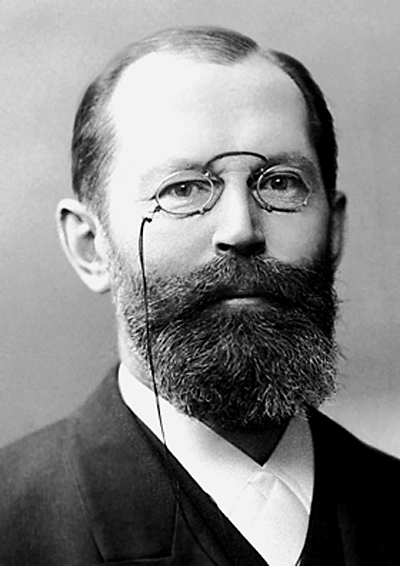
\includegraphics[width=\linewidth]{images/book3/fischer.jpg}
\end{minipage}\hfill
\begin{minipage}[t]{0.78\linewidth}
\vspace{0pt}
एमिल फ़िशर ने 1891 तक ग्लूकोस और उसके समावयवियों के विन्यास निकाल लिए, उससे पहले कि कोई
भौतिक विधि किसी अणु को देख पाती: शर्कराओं को एक-दूसरे में बदलकर और प्राप्त
त्रिविम समावयवियों को गिनकर। उनके द्वारा आविष्कृत प्रक्षेप, जिससे वे उन्हें लिखते थे, आज भी उनका नाम धारण करता है। उन्होंने
पहले संश्लेषित \omterm{def:b2:biomolecules:peptide}{पेप्टाइड} भी बनाए, और उन्हें 1902 का रसायन का नोबेल पुरस्कार मिला। (चित्र: अटेलियर
विक्टोरिया, बर्लिन, लगभग 1895, सार्वजनिक अधिकार-क्षेत्र; विकिमीडिया कॉमन्स।)
\end{minipage}
\end{history}

\section{अभ्यास}

\begin{exercise}[$\star$]\label{exo:b2:biomolecules:1}
ऐलानीन को \omterm{def:b2:biomolecules:amino-acid}{उभयाविष्ट आयन} के रूप में खींचिए, फिर वे रूप जो pH 1 और pH 12 पर प्रभावी हैं।
\end{exercise}

\begin{exercise}[$\star$]\label{exo:b2:biomolecules:2}
ग्लाइसीन का \omterm{def:b2:biomolecules:amino-acid}{समविभव बिंदु} परिकलित कीजिए, और ऐलानीन का ($\mathrm pK_a$ 2.35 और 9.87)।
\end{exercise}

\begin{exercise}[$\star$]\label{exo:b2:biomolecules:3}
डाइपेप्टाइड Ala--Gly खींचिए और उसके \omterm{def:b2:biomolecules:peptide}{पेप्टाइड आबंध} पर घेरा बनाइए। यह Gly--Ala से कैसे भिन्न है?
\end{exercise}

\begin{exercise}[$\star$]\label{exo:b2:biomolecules:4}
शीर्ष पर \ce{COOH} और नीचे \omterm{def:b2:biomolecules:amino-acid}{पार्श्व शृंखला} \ce{CH2OH} वाले फ़िशर प्रक्षेप में सेरीन का
\ce{NH2} बाईं ओर इंगित करता है। यह D है या L? इसका CIP वर्णनक दीजिए।
\end{exercise}

\begin{exercise}[$\star\star$]\label{exo:b2:biomolecules:5}
pH 1, 7 और 12 पर ट्राइपेप्टाइड Lys--Gly--Asp का शुद्ध आवेश दीजिए।
\end{exercise}

\begin{exercise}[$\star\star$]\label{exo:b2:biomolecules:6}
\omterm{def:b2:biomolecules:peptide}{पेप्टाइड आबंध} बनाने के लिए, थायोनिल क्लोराइड से बने और गर्म किए गए रक्षित ऐमीनो
अम्ल के \omterm{def:b2:acyl-substitution:derivative}{ऐसिल क्लोराइड} के बजाय, \omterm{def:b2:biomolecules:peptide}{युग्मन अभिकर्मक} क्यों प्रयुक्त होता है?
\end{exercise}

\begin{exercise}[$\star\star$]\label{exo:b2:biomolecules:7}
D-फ़्रक्टोस अपने C5 \ce{OH} द्वारा C2 कीटोन पर चक्रीकृत होता है। वलय का आकार दीजिए और
\omterm{def:b2:biomolecules:anomer}{हॉवर्थ प्रक्षेप} में $\beta$-D-फ़्रक्टोफ़्यूरैनोस खींचिए।
\end{exercise}

\begin{exercise}[$\star\star$]\label{exo:b2:biomolecules:8}
D-गैलेक्टोस के शुद्ध \omterm{def:b2:biomolecules:anomer}{ऐनोमरों} के विशिष्ट घूर्णन $+150.7$ ($\alpha$) और $+52.8$ ($\beta$) हैं और
साम्य मिश्रण का $+80.2$ (अभ्यास के आँकड़े)। साम्य संघटन परिकलित कीजिए।
\end{exercise}

\begin{exercise}[$\star\star$]\label{exo:b2:biomolecules:9}
समझाइए कि माल्टोस फ़ेलिंग विलयन का अपचयन क्यों करता है और सुक्रोस क्यों नहीं, और तनु अम्ल के साथ गर्म करने के
बाद सुक्रोस क्यों करता है।
\end{exercise}

\begin{exercise}[$\star\star\star$]\label{exo:b2:biomolecules:10}
किसी वसा का \omterm{def:b2:acyl-substitution:saponification}{साबुनीकरण} मान पोटैशियम हाइड्रॉक्साइड का mg में वह द्रव्यमान है जो उसके 1~g का \omterm{def:b2:acyl-substitution:saponification}{साबुनीकरण} करता है।
ट्राइओलीन, \ce{C57H104O6}, के लिए इसे परिकलित कीजिए, और समझाइए कि छोटी शृंखलाओं वाली वसा का मान अधिक क्यों होता है।
\end{exercise}

\begin{exercise}[$\star\star\star$]\label{exo:b2:biomolecules:11}
ग्लाइसीन और ऐलानीन से Gly--Ala के संश्लेषण की योजना बनाइए: रक्षी समूह, सक्रियण, युग्मन,
विरक्षण, एक लांबिक युग्म के साथ।
\end{exercise}

\begin{exercise}[$\star\star\star$]\label{exo:b2:biomolecules:12}
5$'$-ATGCGT-3$'$ का पूरक रज्जुक, उसके 5$'$ सिरे से, लिखिए, और द्वि-रज्जुक को थामे रखने वाले हाइड्रोजन
आबंधों को गिनिए।
\end{exercise}

\section{समस्या: ऐस्पार्टेम}

\begin{problem}[{सप्ताहांत समस्या --- दोनों ऐमीनो अम्ल और उनके विन्यास, pH के विरुद्ध
डाइपेप्टाइड का आवेश, उसका संश्लेषण और $\alpha$/$\beta$ समस्या, और किसी शीतल पेय में
उसका जल-अपघटन}]
\label{pb:b2:biomolecules:1}
ऐस्पार्टेम उस डाइपेप्टाइड का मेथिल एस्टर है जो L-ऐस्पार्टिक अम्ल के $\alpha$-कार्बोक्सिलिक समूह और
L-फ़ेनिलऐलानीन के ऐमीनो समूह से बनता है। आँकड़े: ऐस्पार्टिक अम्ल के $\mathrm pK_a$ 2.0, 3.9 और 9.9 (डाइपेप्टाइड के
समूहों के लिए मॉडल मान)। मोलर द्रव्यमान (\unit{g/mol}): C 12.011, H 1.008, N 14.007,
O 15.999।
% ledger: use:aspartame, pka:asp1, pka:asp2, pka:asp3, aw:C, aw:H, aw:N, aw:O

\medskip
\noindent\textbf{भाग I --- दोनों ऐमीनो अम्ल।}
\begin{enumerate}
  \item ऐस्पार्टेम के पूर्ण जल-अपघटन से मुक्त होने वाले तीन यौगिकों के नाम बताइए।
  \item फ़िशर प्रक्षेप में L-ऐस्पार्टिक अम्ल और L-फ़ेनिलऐलानीन खींचिए।
  \item हर त्रिविमजनक केंद्र का CIP वर्णनक दीजिए।
  \item ऐस्पार्टेम के कितने त्रिविम समावयवी हैं?
  \item ऐस्पार्टेम खींचिए और \omterm{def:b2:biomolecules:peptide}{पेप्टाइड आबंध} और एस्टर चिह्नित कीजिए।
  \item मीठे स्वाद के लिए हर ऐमीनो अम्ल का विन्यास क्यों महत्त्वपूर्ण है?
\end{enumerate}

\medskip
\noindent\textbf{भाग II --- pH के विरुद्ध आवेश।}
\begin{enumerate}[resume]
  \item ऐस्पार्टेम के आयननीय समूहों की सूची बनाइए। C-अंत्य उनमें से एक क्यों नहीं है?
  \item मॉडल मानों से pH 2 पर शुद्ध आवेश दीजिए।
  \item pH 7 पर वही।
  \item pH 12 पर वही।
  \item इस मॉडल में \omterm{def:b2:biomolecules:amino-acid}{समविभव बिंदु} का अनुमान लगाइए।
  \item डाइपेप्टाइड के वास्तविक $\mathrm pK_a$ मान मुक्त ऐस्पार्टिक
        अम्ल के मानों से भिन्न क्यों होंगे?
\end{enumerate}

\medskip
\noindent\textbf{भाग III --- संश्लेषण।}
\begin{enumerate}[resume]
  \item ऐस्पार्टिक अम्ल और फ़ेनिलऐलानीन के मेथिल एस्टर को केवल साथ गर्म क्यों नहीं किया जा सकता?
  \item ऐस्पार्टिक अम्ल के किन समूहों का रक्षण आवश्यक है?
  \item \omterm{def:b2:biomolecules:peptide}{युग्मन अभिकर्मक} मुक्त कार्बोक्सिलिक समूह के साथ क्या करता है?
  \item ऐस्पार्टिक अम्ल के दो कार्बोक्सिलिक समूह हैं। यदि ग़लत समूह युग्मित हो जाए तो क्या बनता है?
  \item ऐसा लांबिक रक्षण प्रस्तावित कीजिए जो केवल $\alpha$-कार्बोक्सिलिक समूह को मुक्त छोड़े, और उसका
        निष्कासन।
  \item सक्रियित ऐमीनो अम्ल को क्षारीय परिस्थितियों में बहुत देर तक क्यों नहीं छोड़ना चाहिए?
  \item चरणों का अनुक्रम लिखिए।
\end{enumerate}

\medskip
\noindent\textbf{भाग IV --- शीतल पेय में जल-अपघटन।}
\begin{enumerate}[resume]
  \item किसी अम्लीय पेय में ऐस्पार्टेम के कौन-से आबंधों का जल-अपघटन हो सकता है? कौन-सा पहले?
  \item केवल एस्टर के जल-अपघटन के उत्पाद दीजिए।
  \item पुराना पेय कम मीठा क्यों लगता है?
  \item ऐस्पार्टेम, \ce{C14H18N2O5}, का मोलर द्रव्यमान परिकलित कीजिए।
  \item \qty{180}{mg} वाले एक डिब्बे में ऐस्पार्टेम की मात्रा परिकलित कीजिए।
  \item ऐस्पार्टेम के \qty{180}{mg} के पूर्ण जल-अपघटन से मुक्त मेथेनॉल का द्रव्यमान
        बताइए।
\end{enumerate}
\end{problem}
